% !TEX root = ../main.tex
\begin{linenumbers}

\section{Archer Kin}
\DndDropCapLine{W}{hile traversing the jungle, be very}
\textit{conscious of your surroundings.
If you stumble upon fiber nests in the trees.
If you hear childlike voices screaming.
Run.
Run as fast as you can.}

\hspace*{\fill} --- Hedwyn's guide to the Chirping Wilds.

The archer kin are a species that resemble large marmosets, barely reaching 90 cm of height.
They share the brown coloration, white ears, and striped tail.
They are small creatures that inhabit the rivers, forests, and jungles of Yuadrem.

They are also known as marsets, or yuathe tle'thal rlue in Jantherlin.
Apart from their size, the other difference from marmosets is their back, which is protected by elongated, pointed quills, used as arrows.

Marsets are an asexual species able to lay eggs at necessity via a ritual after reaching maturity, only limited by the amount of dwellings and social constraints.

\subsection*{Misleading Appearance}
Marsets don't seem terribly intimidating at first glance.
They however have an unusual defense mechanism for driving away threats, which includes any unfortunate creature that disturbs their large arboreal colonies.

Each marset grows specialized quills from their back, with a smooth tip and a base with four flanges, like the fletching of an arrow.
In additional to making the marsets quite painful to grab, these quills are used as projectiles.

The little creatures construct their own bows, stripping bark from bendy twigs with their teeth to create the limbs, and harvesting spiderweb for the string.
The strands are rubbed together with sand, which is done to thicken the bowstring and reduce stickiness in the middle, creating a sophisticated weapon to launch quills at unlucky foes.

For shorter range, marsets also use hollow reeds to blow their quills as darts.
It's common for the smarter marsets to apply manure or poison to their arrows and darts, improving their deadliness.

\begin{figure}[!b]
    \centering
    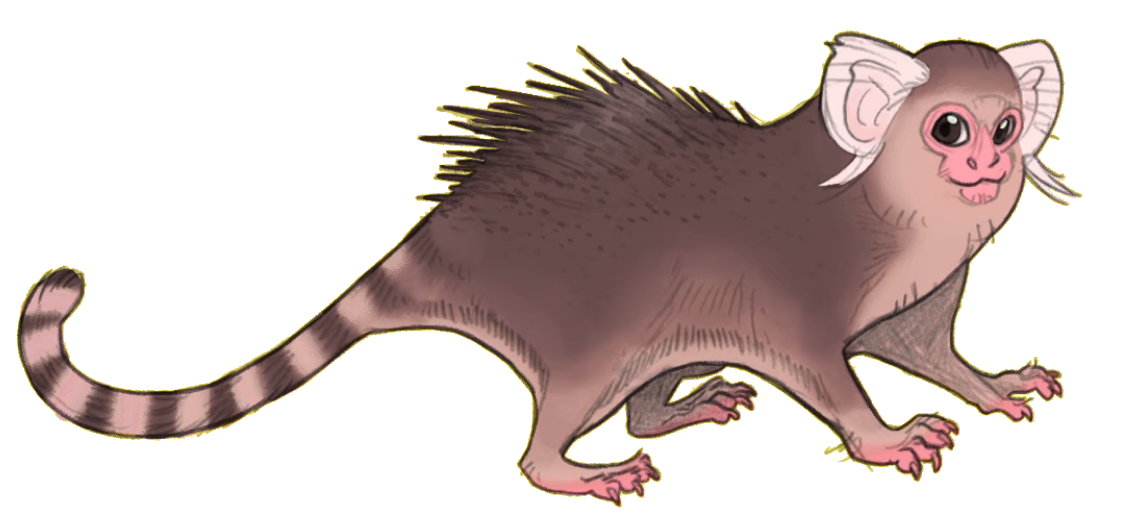
\includegraphics[width=0.48\textwidth]{03kins/img/13marset_brown.png}
\end{figure}

\subsection*{Arboreal Colonies}
The colonies that the marsets protect are just as complex as their weapons.
The structures are created from weaving grass and plant fibres around tree branches to create interconnected chambers.

A single colony can have up to 100 rooms and even more individuals living in it.
Rooms are assigned a specific function, and are passed down through related members of the colony.

Nursery rooms are where marsets lay their eggs, which they hatch into fluffy yellow infants.
Bedrooms are where the adults sleep.
Storage rooms are where food and various items are stockpiled.

In farming rooms they deposit a mixture of tough chewed leaves and bark, which then grows mushrooms.
The little marsets use these rooms to turn otherwise inedible foraged material into something tender and tasty.

While most marsets can be found in these colonies, some choose to live in cities and towns from other civilizations.
Here, they usually build interconnected rooms in trees, creating microcosms of the larger colonies.
Despite their fierceness in their natural environment, marsets are generally regarded as friendly creatures when encountered in urban settings.

\begin{figure}[!t]
    \centering
    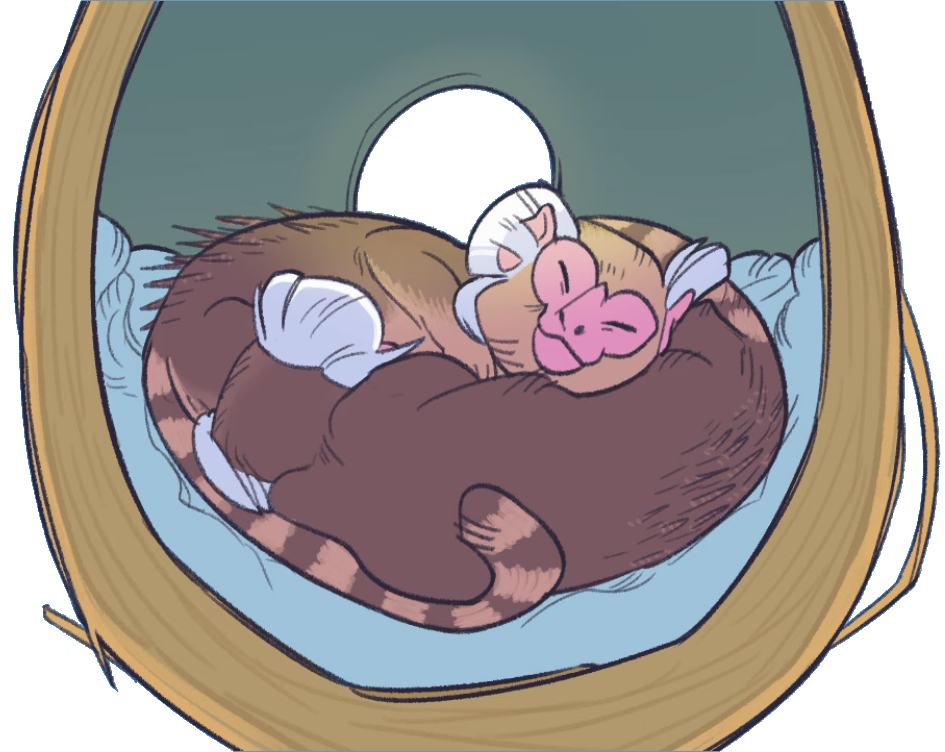
\includegraphics[width=0.48\textwidth]{03kins/img/13marset_room.png}
\end{figure}

\subsection*{Repetitive Language}
Marsets hatch from their eggs already able to speak a strange repetitive language, which is entirely regular and does not evolve.
This language --- known as Babazano --- can be spoken in one of two ways: soundlessly, with the communication happening through lip reading, or screamed as loud as possible, with no middle ground.
Despite this, a marset can learn other languages and not constantly scream at the top of their lungs, but they do tend to be loud speakers.

Babazano has only ten consonants.
All verbs use a single consonant as their root, so there's only ten verbs.
By repeating syllables they create new meanings, which makes their language very difficult to understand by the other kins, but for these little creatures it's no issue at all.
They hear or lip-read a word and instinctively know which one it is.

\subsection*{Exploring Opportunities}
Marsets don't usually set out on the adventurer's path for leisure, but rather out of necessity.
They will only leave their colonies to defend their communities or support their friends.
Only very few will set out to explore the wide world.
% For them, adventuring is less a career than an opportunity and more of a necessity.

\begin{figure}[!t]
    \centering
    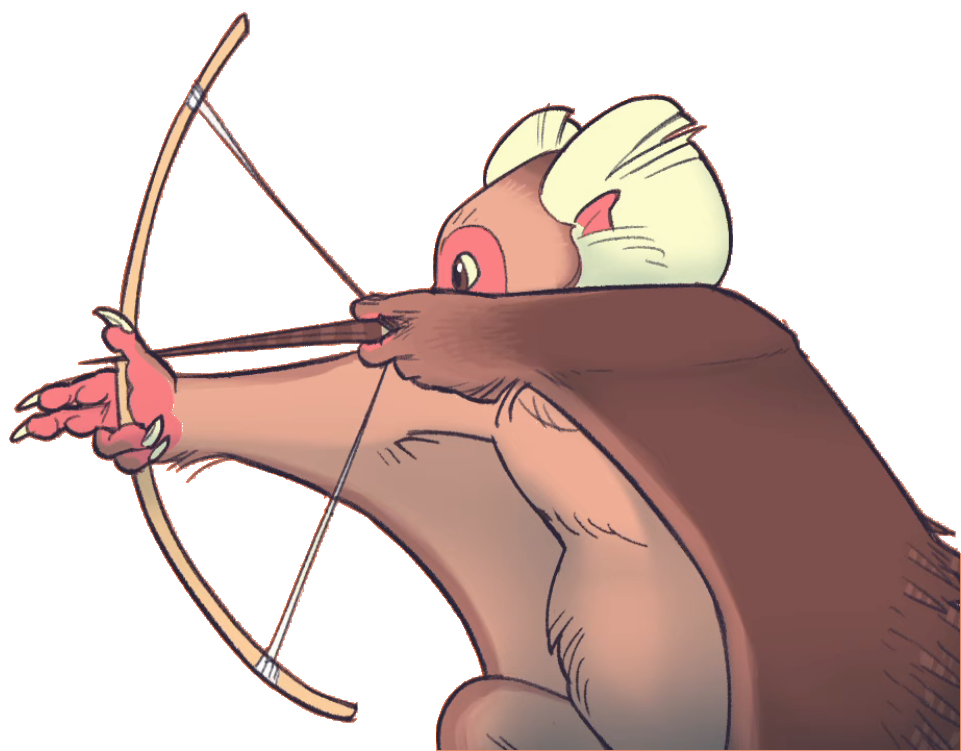
\includegraphics[width=0.48\textwidth]{03kins/img/13marset_bow.png}
\end{figure}

\subsection*{Marset Names}
Marsets assign names to each other based on distinctive features and accomplishment.
An individual marset will wear many names during their childhood, and when they settle on one is when they reach adulthood.
Due to the peculiarity of Babazano, it is a common for the other kins to call them by simple monikers, practice that the marsets despise.
% Most marsets don't particularly like this, and are very reluctant to accept a nickname given to them.

\paragraph{Names} Do Anana, Do Baba, Do Badada, Do Ebebebebe, Do Ezeze, Do Nono, Do Odododo, Do Uvu, Do Veve, Do Vovovo.

\subsection*{Traits}
Your marset character has a range of abilities based on its nature and community lifestyle.

\subparagraph{Ability Score Increase} Your Charisma score is increased by 2, and your Dexterity score is increased by 1.

\subparagraph{Age} Marsets has a short lifespan, reaching maturity by age 4 and not living much more than 50 years.

\subparagraph{Alignment} Marsets have a tendency towards helping others, specially in their communities, and are inclined towards the gold tide.

\subparagraph{Size} Marsets range from 75 to 90 cm.
They usually have a slender and agile frame, weighing around 20 kg.
Your size is small.

\subparagraph{Speed} Your base walking speed is 9 meters, and you have a climbing speed of 9 meters.

\subparagraph{Glider} You have loose flaps of furry skin between your arms and legs, which allow you to glide short distances at a speed of 9 meters per turn, as long as you are not wearing heavy armor.
You fall at a rate of 6 meters per turn while gliding, and suffer no falling damage on landing.

\subparagraph{Sneaky Nature} You have advantage on stealth checks in heavily forested areas.

\subparagraph{Natural Weapons} You are proficient with shortbows and blowguns, and can use your own quills as arrows or cut them to be used as darts.
Every day you can gather up to 10 quills from your back to be used in this fashion.

\subparagraph{Community lifestyle} Despite their loudness, marsets can be very compelling talkers.
You are competent in the Persuasion skill.

\subparagraph{Languages} You can speak Babazano from birth, and can lip-read the language.
You are also able to read and write Leafrunes, a special writing system designed to communicate simple messages to others of your kin.
Additionally, you know how to speak a language of your choice, but you don't know how to read or write it.

\begin{figure}[!b]
    \centering
    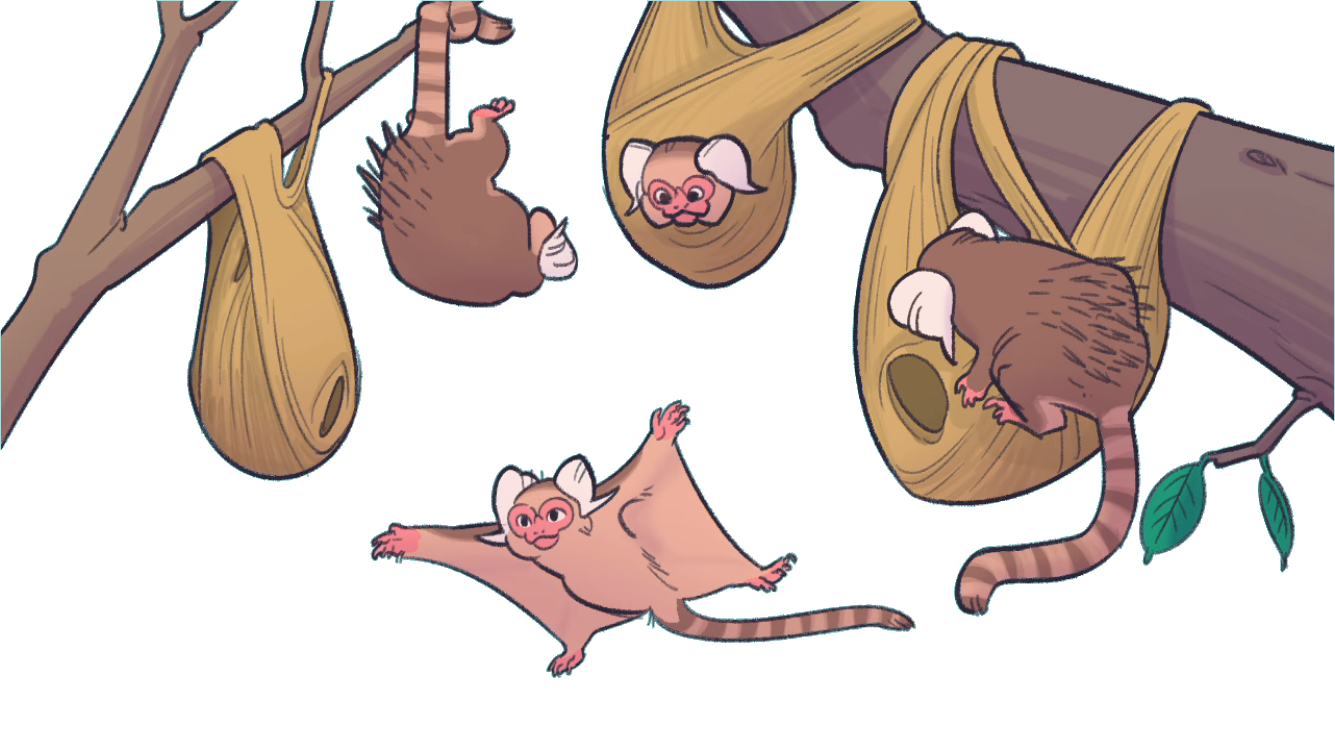
\includegraphics[width=0.48\textwidth]{03kins/img/13marset_colony.png}
\end{figure}
\end{linenumbers}

\newpage
